\documentclass[11pt]{article}
\usepackage{amsmath}
\usepackage{graphicx}
\usepackage{layout}
\usepackage{gensymb}
\usepackage{caption} 
\usepackage{subcaption}
\usepackage{hyperref}

%Paper formatting stuff
\RequirePackage[letterpaper]{geometry}	%USLetter = standad paper.
\textheight = 615pt 
\textwidth = 470pt
\oddsidemargin = 0pt
\marginparwidth = 60pt
\marginparsep = 12pt
\marginparpush = 0pt %Not shown
\topmargin = 0pt
\headheight = 0pt
\headsep = 0pt 
\footskip = 36pt
\pagestyle{plain}

\title{\textbf{GEANT4 Simulation of the Jlab MeV Mott Polarimeter}}
\author{Martin McHugh\\
		The George Washington University\\
		mjmchugh@jlab.org}
\date{2015-07-01}
\begin{document}

\maketitle

\begin{abstract}
The simulation of the JLab Mott Polarimeter accurately simulates single scattering and the detector response thereof. Results are shown for this case. Additionally, work is being done to simulate realistic double scattering. Preliminary results and methods attempted are described. 
\end{abstract}

\section{JLab Polarimeter and Mott Scattering}

The MeV Mott Polarimeter is located in the Continuous Electron Beam Accelerator Facility (CEBAF) injector at Jefferson Lab (JLab). It is used to measure the transverse polarization of the electron beam in the 2 - 10 MeV energy range. The polarimeter measures the elastic scattering asymmetry of electrons incident on the nuclei of a thin target foil. The foils used include gold, silver, and copper and range in thickness from 100-10,000 \AA. The elastically scattered electrons pass through aperatures of an aluminum collimator that defines the scattering angle of 172.6$^\circ$ $ \pm$ 0.1$^\circ$ with a per quadrant solid angle of 0.18 msr. The scattered electrons pass then pass through the 0.2032 mm (8 mil) thick aluminum window and into the detector packages. Each detector package contains two plastic scintillators connected to PMTs for readout: a 1 mm $\times$ 25.4 mm $\times$ 25.4 mm wafer scintillator, the $\Delta$ E detector, and a cylindrical 76.2 mm diameter, 63.5 mm long scintillator, the E detector, which functions as a stop detector and calorimeter with a 3\% energy resolution. All of this equipment is modelled in the \texttt{GEANT4} simulation and the geometries implemented can be found in \texttt{MottDetectorConstruction.cc}.

\subsection{Mott Scattering}

The polarimeter functions by measuring the Mott scattering asymmetry. Mott scattering describes elastic electron-nuclear scattering. The differential cross-section can be written as
\begin{equation}
 \frac{d\sigma}{d\Omega}(\theta) = I(\theta)\left(1 + S(\theta)\vec{P}\cdot\hat{n}\right)
\end{equation}
where $I(\theta)$ is the spin independent form of the Mott cross section, $\vec{P}$ is the incoming beam's polarization, $S(\theta)$ is known as the Sherman function and 
\begin{equation}
 \vec{n} = \frac{\vec{p}\times\vec{p}^{\,\prime}}{\left|\vec{p}\times\vec{p}^{\,\prime}\right|}
\end{equation}
where $\vec{p}$ ($\vec{p}^{\,\prime}$) is the incoming (outgoing) momentum of the electron. In the case of ideal single scattering we expect to measure an asymmetry,
\begin{equation}
 \label{eq:SimpleAsym}
 A = \frac{N_L-N_R}{N_L+N_R} = P_yS(\theta_{sc})
\end{equation}
where $N_{L(R)}$ is the number of hits in the left(right) detector placed at a scattering angle, $\theta_{sc}$. However, the asymmetry we actually observe depends on target thickness and is averaged over the acceptance of our detectors. This produces an ``effective" Sherman function, $S_{eff}(\theta,d\Omega,d)$, where $d\Omega$ is the detector acceptance and $d$ is the target thickness. The solid angle is fixed for the polarimeter and can be dealt with by averaging the Sherman function over the acceptance. The target thickness dependence is clearly shown in Fig. \ref{fig:DataVsSingleSim}. This target thickness dependence is suspected to be due to electrons that undergo multiple Mott scatterings within our target. The goal of the \texttt{GEANT4} simulation is to see if we can reproduce the effective Sherman function in order to verify our polarimeter's accuracy.   

\begin{figure}[!h]
 \centering
 \includegraphics[width=0.5\textwidth]{Plots/DataSimAsymVsThickness.pdf}
 \caption{Comparison of measurements (blue crosses) with single scattering simulation (orange diamonds). All error bars are smaller than the points. Simulated results have been scaled to assume $P = 89\%$ to match the polarization at which the data was taken.} 
\label{fig:DataVsSingleSim}
\end{figure}

\subsection{Double Mott Scattering}
It is our assumption that the target thickness dependence of the Mott scattering asymmetry is the result of multiply scattered electrons within the target foil. Simulation of this effect requires us to track the polarization over multiple steps. A Mott scattered electron beam carries a new polarization. 
\begin{equation}
 \vec{P}^\dagger = \frac{\left(\vec{P}\cdot\vec{n}+S(\theta)\right)\vec{e}_1 + U(\theta)\vec{e}_2 + T(\theta)\vec{e}_3}{1+\vec{P}\cdot\vec{n}\,S(\theta)} 
\end{equation}
where
\begin{eqnarray}
 \vec{e}_1 &=& \vec{n} \\
 \vec{e}_2 &=& \vec{n}\times\vec{P} \\
 \vec{e}_3 &=& \vec{n}\times\left(\vec{P}\times\vec{n}\right)
\end{eqnarray}
and $U(\theta)$ and $T(\theta)$ are functions which measure the spin transfer probability of the scattering. Plots of the relevant scattering functions for a selection of typical energies can be seen in Fig. \ref{fig:ScatteringFunctions}. Those four plots are generated using the scattering calculations performed by Xavier Roca Maza on 2015-05-29. These calculations form the basis of Mott scattering physics in our simulation. One can observe that the JLab Mott Polarimeter was built at the point where the asymmetry is largest rather than at the point where the figure of merit (shown in Fig. \ref{fig:FoM}) is maximized. 

\begin{figure}[!h]
\begin{subfigure}{.5\textwidth}
  \centering
  \includegraphics[width=.8\linewidth]{Plots/Mott_Au_CrossSection.pdf}
  \label{fig:CrossSec}
\end{subfigure}
\begin{subfigure}{.5\textwidth}
  \centering
  \includegraphics[width=.8\linewidth]{Plots/Mott_Au_ShermanFunction.pdf}
  \label{fig:ShermanFunction}
\end{subfigure}\\
\begin{subfigure}{.5\textwidth}
  \centering
  \includegraphics[width=.8\linewidth]{Plots/Mott_Au_SpinT.pdf}
  \label{fig:SpinT}
\end{subfigure}
\begin{subfigure}{.5\textwidth}
  \centering
  \includegraphics[width=.8\linewidth]{Plots/Mott_Au_SpinU.pdf}
  \label{fig:SpinU}
\end{subfigure}
 \caption{Mott physics as a function of angle for typical polarimeter energies.} 
\label{fig:ScatteringFunctions}
\end{figure}

\begin{figure}[!h]
 \centering
 \includegraphics[width=0.5\textwidth]{Plots/Mott_Au_FoM.pdf}
 \caption{Figure of Merit, $I(\theta)S(\theta)^2$, for typical polarimeter energies.} 
\label{fig:FoM}
\end{figure}

\subsection{Previous Efforts}
In the past, Michael Steigerwald, performed a direct integration of the form:
\begin{equation}
N = \int\limits_{\theta = 0}^{\pi} \int\limits_{\phi = 0}^{2\pi} \int\limits_{x_1 = 0}^{D} \int\limits_{\psi=\theta_{2}}^{\theta_2+\Omega_\theta}\sigma_1(x_1,\theta, \phi)\sigma_2(x_2,\theta_2)E(x_1,x_2) d\psi dl d\phi d\theta.
\end{equation}
and obtained a resulting thickness dependence of the Sherman Function to be:
\begin{equation}
S(d) = S(0)\frac{1 + 0.00272d^{0.866}}{1 + 0.23d^{0.866} + 0.0739d + 0.0146d^2+ 0.00339d^3}.
\end{equation}
Unfortunately, this result has not been reproducible. A summary of his work can be found in \url{https://wiki.jlab.org/ciswiki/images/2/28/AIP570_935_2001.pdf}.

\section{Simulating Mott Scattering}

To begin our simulation, we must generate electrons in our apparatus to represent certain physical cases. Before we discuss the particular cases the simulation can model in the following sections, we look at the properties of our ``incident beam'' of electrons on the target. 

In all of the following cases, the electron beam is assumed to have an initial polarization. While the user may modify this, the standard assumption made is that the beam is 100\% polarized in the positive $y$ direction; $\vec{P}_1 = \hat{j}$. The incident electrons are assumed to have momentum entirely in the $z$ direction; $\vec{p}_1 = p \hat{k}$. Finally, the beam is assumed to have a circular, Gaussian profile on the target with a width of 1 $\mu$m. All of the exact methods can be found in \texttt{MottPrimaryGeneratorAction.cc}.

\subsection{Single Scattering}
To look at the detector response to electrons that undergo exactly one Mott scattering process in the target, we use the following algorithm:
\begin{enumerate}
 \item Pick a scattering position, $\vec{x}_1$, within the intersection of the beam and our target.
 \item Pick a point, $\vec{x}_2$, in the acceptance the primary collimator.
 \item Calculate $\frac{d\sigma}{d\Omega}(\vec{x}_1,\vec{x}_2)$.
 \item Rejection sample against this cross-section. If accepted, proceed to generate the event. If rejected repeat steps 1-3.  
\end{enumerate}
The simulations shown herein all assume 100\% polarization in the $y$ direction and look only at 5 MeV electrons. In order to measure the Mott asymmetry from single scattering simulations, we simply use Eq. (\ref{eq:SimpleAsym}):
\begin{equation}
 A = \frac{N_L-N_R}{N_L+N_R} = -0.513 \pm 0.0005
\end{equation}
Unfortunately, the results do not change with target thickness as shown in Fig. \ref{fig:DataVsSingleSim} (Note that the simulation results have been scaled to assume that $P = 89\%$). This confirms that single scattering is not adequate to explain the results of thick target foils. Typical spectra from this event generator can be seen in Fig. \ref{fig:SimSinglevsDouble}.

\begin{figure}[!h]
 \centering
 \includegraphics[width=\textwidth]{Plots/SimulatedSpectra.pdf}
 \caption{Simulated normalized single (double) scattering spectra in blue (red). It is clear that double scattering contributes non-trivially to both the peak and to the shoulder, however rate calculations need to be performed to quantify the contribution accurately.} 
\label{fig:SimSinglevsDouble}
\end{figure}

\subsection{Double Scattering: First Method}

The first method I've used to calculate the effect of double scattering is as follows,
\begin{enumerate}
 \item Pick a scattering position, $\vec{x}_1$, within the intersection of the beam and our target.
 \item Pick a point, $\vec{x}_2$, within the target, such that $|\vec{x}_2-\vec{x}_1| <$ 0.16 mm. Beyond this distance in Gold a 5 MeV electron will lose over 500 keV and no longer be of interest to us.    
 \item Calculate $\frac{d\sigma_1}{d\Omega_1}(\vec{x}_1,\vec{x}_2)$.
 \item Pick a point, $\vec{x}_3$, in the acceptance the primary collimator.
 \item Calculate $\frac{d\sigma_2}{d\Omega_2}(\vec{x}_2,\vec{x}_3)$.
 \item Rejection sample against this $\frac{d\sigma_1}{d\Omega_1}\frac{d\sigma_2}{d\Omega_2}$. If accepted, generate electron at $\vec{x}_2$ towards $\vec{x}_3$  If rejected repeat steps 1-5.
\end{enumerate}
This method produces an asymmetry of $\boxed{A = -0.0111 \pm 0.0005}$. Unfortunately this asymmetry also does not scale with target thickness. Simulated spectra from this generator can be seen in Fig. \ref{fig:SimSinglevsDouble}. Scattering vertex information from this method can be seen in Fig. \ref{fig:DoubleScattering}.

\begin{figure}[!h]
\begin{subfigure}{\textwidth}
 \includegraphics[width=0.9\linewidth]{Plots/Left_2_Scattering.pdf}
\end{subfigure}\\
\begin{subfigure}{\textwidth}
 \includegraphics[width=0.9\linewidth]{Plots/Right_2_Scattering.pdf}
\end{subfigure}
 \caption{Double scattering information for hits in each detector. From left to right in the top row, the initial cross-section, scattering angle, and azimuthal angle. The bottom row contains the same information for the second scattering.}
\label{fig:DoubleScattering}
\end{figure}

The second method attempted to model double scattering is as follows:
\begin{enumerate}
 \item Pick a scattering position, $\vec{x}_1$, within the intersection of the beam and our target.
 \item Pick a direction direction, $(\theta_1,\phi_1)$, from the uniform unit sphere.
 \item Pick a point, $\vec{x}_2$, uniformly between $\vec{x}_1$ and the edge of the foil (or 0.16 mm as in the previous example).
 \item Pick a point, $\vec{x}_3$, in the acceptance the primary collimator.
 \item Throw from $\vec{x}_2$ towards $\vec{x}_3$.
\end{enumerate}
This method does not rejection sample as the previous two do but it may allow for calculation of rates if the proper integral can be performed. 

\begin{figure}[!h]
 \includegraphics[width=\textwidth]{Plots/DoubleScattering.pdf}
\end{figure}

\subsection{Calculating Rates}
The basic equation for linking the simulation with data applies to total scattering rate detected,
\begin{equation}
 \mathcal{R} = \mathcal{L} \int_x \sigma(x)\epsilon(x)
\end{equation}
where $\mathcal{R}$ is the scattering rate in the detector, $\sigma$ is the cross section, $\epsilon$ is the effective solid angle of the detector, $\mathcal{L}$ is the luminosity and, $x$ represents the various degrees of freedom over which the integral is done. The GEANT4 package is used to do the implicit integral over degrees such as target position and various external processes (transportation and scattering outside of the target etc.). 

\subsubsection{Single Scattering Rates}
In the case of single scattering, the above equation becomes:
\begin{equation}
 R = \mathcal{L} \int_0^{2\pi}\int_{-1}^1 \sigma(\theta,\phi)\rho (\theta,\phi)d\cos\theta d\phi
\end{equation}
where $\rho(\theta,\phi)$ is the probability of an event making it into the detector in simulation. We can approximate this integral simply:
\begin{equation}
 \mathcal{R} \approx \mathcal{L} \left\langle\frac{d\sigma}{d\Omega}\right\rangle_{hits} \Delta\phi \Delta\cos\theta \frac{N_{hit}}{N_{thrown}}
\end{equation}
To test the accuracy of this method, simulations were run using angular ranges of $\phi \in [-10^\circ,10^\circ]$ centered around the appropriate collimator hole (left or right) and $\theta \in [170^\circ,175^\circ]$. Results from runs of 100,000 events for each detector at both 0.05 $\mu$m and 1.0 $\mu$m targets are shown in Table \ref{table:SimulatedRates}. It appears that single scattering accounts for $\approx 90\%$ of the signal observed from our thinnest target and $\approx 80\%$.

\begin{table} [h!]
 \centering
 \begin{tabular}{| c | c | c | c | c |} 
  \hline d (nm) & $\mathcal{R}_L$ (Hz/$\mu$A) & $\mathcal{R}_R$ (Hz/$\mu$A) & $\mathcal{R}_\mathrm{avg}$ & $\mathcal{R}_\mathrm{data}$ \\
  \hline 50 & 4.88 $\pm$ 0.11 & 15.02 $\pm$ 0.32 & 9.95 $\pm$ 0.17 & 9.4 $\pm$ 0.1\\
  \hline 225 & 22.27 $\pm$ 0.49 & 69.22 $\pm$ 1.48 & 45.74 $\pm$ 0.78 & 41.5 $\pm$ 0.5\\
  \hline 350 & 34.47 $\pm$ 0.76 & 104.70 $\pm$ 2.31 & 69.58 $\pm$ 1.21 & 71.5 $\pm$ 1.0\\  
  \hline 1000 & 104.3 & 241.9 & 173.1 & 214.3 \\
  \hline
 \end{tabular}
 \caption{Simulated rates for single scattering in the left and right detectors for our thinnest and thickest typical foils. Data averaged from \url{https://wiki.jlab.org/ciswiki/images/4/47/Analysis_Slides_7_29.pdf}}
 \label{table:SimulatedRates}
\end{table}

\subsubsection{Double Scattering Rates}

In the case of double scattering, it's not immediately apparent how to calculate the rates since the form of $\epsilon(x)$ is much more complicated. We begin by imagining scattering from one point in the target $\vec{x}_1$ to another $\vec{x}_2$. The rate of scattering from an infinitesimal volume about $\vec{x}_1$ towards an infinitesimal solid angle around $\vec{x}_2$ is 
\begin{equation}
d\mathcal{R}_{1\rightarrow2}(\vec{x}_1,\vec{x}_2) = n_b(\vec{x}_1) \frac{N_A\rho_m}{A} \sigma_1(\vec{x}_1,\vec{x}_2)dx_1dy_1dz_1d\Omega_1
\end{equation}
In the next step, we must consider the scattering from point $\vec{x}_2$ into our acceptance in direction $(\theta,\phi)\in(\theta_{sc}\pm\delta\theta,\phi_{sc}\pm\delta\phi)$. The differential should be
\begin{equation}
d\mathcal{R}_\Omega(\vec{x}_1,\vec{x}_2) = d\mathcal{R}_{1\rightarrow2}(\vec{x}_1,\vec{x}_2)\frac{N_A\rho_m}{A} d'(\vec{x}_1) \sigma_2(\vec{x}_1,\vec{x}_2,\theta,\phi) \rho(\theta,\phi) d\Omega
\end{equation}
We must find a method of numerically integrating this quantity over all of the volume of the foil and over the detectors acceptance. 

We first consider the case of double scattering by discussing the variables upon which a double scattering event depends. The rate of electrons scattered from the first point along a certain direction depends upon the following variables: Initial energy, $E$, scattering position, $\vec{x} = (x,y,z)$, and scattering angle, $(\theta,\phi)$. The second scattering also depends upon these but additionally depends upon the following: the distance travelled inside the target foil, $\zeta$, and the global angles of the particles outgoing momentum, $(\Theta,\Phi)$.


\section{Conclusions}

The \texttt{GEANT4} simulation of the JLab MeV Mott Polarimeter is a useful tool. So far it has produced single scattering results which have an asymmetry consistent with measurements extrapolated to zero target thickness and rates which are within 10-20\% of the measured values. Work is ongoing in two areas: producing an event generator which can accurately predict the asymmetry of double scattered electrons, calculating rates for double scattered electrons to determine the extent to which they dilute the single scattering signal. 

\end{document}

\usepackage{tikz}
\usetikzlibrary{%
    decorations.pathreplacing,%
    decorations.pathmorphing%
}
\usepackage{verbatim}

\begin{comment}
:Title: Oblique Incidence
:Tags: Decorations, Physics & chemistry

Reflection and refraction of electromagnetic waves incident obliquely at plane interface. 

:Author: `Edgar Fuentes`_

.. _Edgar Fuentes: http://groups.google.co.ve/group/LaTeXuC

\end{comment}


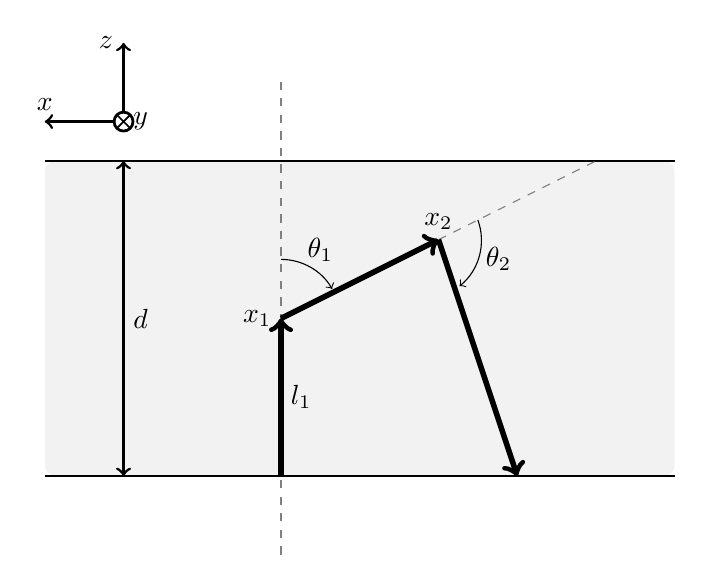
\begin{tikzpicture}[
    media/.style={font={\footnotesize\sffamily}},
    wave/.style={
        decorate,decoration={snake,post length=1.4mm,amplitude=2mm,
        segment length=2mm},thick},
    interface/.style={
        % The border decoration is a path replacing decorator. 
        % For the interface style we want to draw the original path.
        % The postaction option is therefore used to ensure that the
        % border decoration is drawn *after* the original path.
        postaction={draw,decorate,decoration={border,angle=-45,
                    amplitude=0.3cm,segment length=2mm}}},
    ]
    
    % Target Foil
    % Round rectangle
    \fill[gray!10,rounded corners] (-4,-2) rectangle (4,2);
    \draw[black,line width=.5pt](-4,2)--(4,2);
    \draw[black,line width=.5pt](-4,-2)--(4,-2);
    % Vertical dashed line
    \draw[dashed,gray](-1,-3)--(-1,3);
    % target thickness
    \draw[<->,line width=1pt] (-3,-2)--(-3,2);
    \draw(-3,0)node[right]{$d$};

    % Coordinates system
    \draw(-3,2.5)node[right]{$y$};
    \draw[<->,line width=1pt] (-4,2.5) node[above]{$x$}-|(-3,3.5) node[left]{$z$};
    \filldraw[fill=white,line width=1pt](-3,2.5)circle(.12cm);
    \draw[line width=.6pt] (-3,2.5)
                          +(-135:.12cm) -- +(45:.12cm)
                          +(-45:.12cm) -- +(135:.12cm);
    
    % First Path
    \draw[->,line width=2pt] (-1,-2)--(-1,0);    
    \draw(-1,-1)node[right]{$l_1$};
    \draw(-1,0)node[left]{$x_1$};    
    % Second Path
    \draw[->,line width=2pt] (-1,0)--(1,1);    
    \draw(1,1)node[above]{$x_2$};
    \draw[dashed,gray](1,1)--(3,2);
    % First Angle
    \path (-1,0)++(60:1cm)node{$\theta_1$};
    \draw[->] (-1,0.75) arc (90:30:.75cm);
    % Third Path
    \draw[->,line width=2pt] (1,1)--(2,-2);
    % Second Angle
    \path (1,1)++(-17.5:0.8cm)node{$\theta_2$};
    \draw[->] (1.5,1.25) arc (20:-51:.75cm);
    
    % To-paths are really useful for drawing curved lines. The above
    % to path is equal to:
    %
    % \draw[-latex,thick](3.2,0.5)node[right]{$\mathsf{S_{1,2}}$}
    %      ..controls +(180:.2cm) and +(up:0.25cm) .. (3,0);
    % Internally the to path is translated to a similar bezier curve,
    % but the to path syntax hides the complexity from the user. 
\end{tikzpicture}